\documentclass[crop,tikz]{standalone}

\usepackage{makecell}
\usetikzlibrary{positioning}

\newcommand{\vvectorSmall}[1]{\tikz{\draw[#1,step=.5em,fill=#1!50] (0,0)  grid (.5em,1.5em) rectangle (0, 0);}}
\newcommand{\vvector}[1]{\tikz{\draw[#1,step=1em,fill=#1!50] (0,0)  grid (1em,4em) rectangle (0, 0);}}

\definecolor{airforceblue}{rgb}{0.36, 0.54, 0.66}
\definecolor{alizarin}{rgb}{0.82, 0.1, 0.26}

\begin{document}

\begin{tikzpicture}

    \node (waveform) {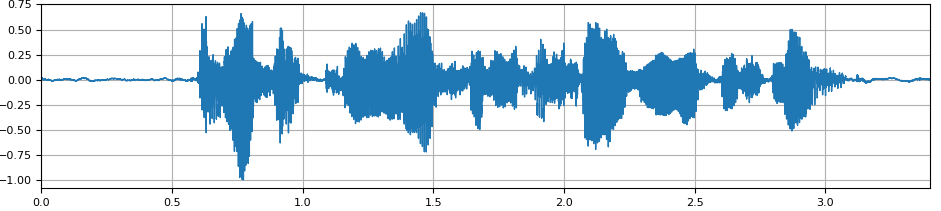
\includegraphics[width=14cm]{waveform.png}};

    \node [above=of waveform, minimum width=15cm, draw=alizarin, rounded corners, line width=2pt, fill=alizarin!50] (transformer) {\makecell{\Large Neural Network \\ (e.g. \texttt{wav2vec2})}};

    \foreach \x in {-6, -4, ..., 4, 6} {
        \draw[->, line width=2pt] ([shift={(\x, 0)}]waveform.north) -- ([shift={(\x, 0)}] transformer.south);
    }
    
    \foreach \x in {-6, -4, ..., 4, 6} {
        \node [above=of transformer, shift={(\x, 0)}] (n\x) {\vvector{airforceblue}};
    }

    \foreach \x in {-6, -4, ..., 4, 6} {
        \draw[->, line width=2pt] ([shift={(\x, 0)}]transformer.north) -- (n\x.south);
    }

\end{tikzpicture}

\end{document}